\section{Data Quality}
\label{sec:quality}

\begin{table}[htbp]
\caption{Data quality of every campaign of \texttt{measured/v3}, from each campaign's data check: first day and span of the journal in hours, runs done, missing, failed, checksum conflicts, runs failing strict validation, runs above the foreign-CPU threshold, configurations under 100 clock ticks, and configurations that trend with the execution order ($|\rho|>0.5$). The grain campaigns pool every grain of a configuration, so their trend count mixes grains. The two counter campaigns of the loop have no data check report; their run count is that of the journal.}\label{tab:quality}
\centering\footnotesize
\begin{tabular}{llrrrrrrrrr}
\toprule
Campaign & Start & Hours & Runs & Miss. & Fail. & Chk. & Strict & CPU & Clock & Trend \\
\midrule
campaign & 2026-11-21 & 14.0 & 5310 & 0 & 0 & 0 & 0 & 0 & 0 & 1 \\
tier & 2026-11-22 & 5.8 & 2100 & 0 & 0 & 0 & 0 & 0 & 0 & 0 \\
perf & 2026-11-22 & 1.8 & 720 & 0 & 0 & 0 & 0 & 0 & 0 & 1 \\
simd-scalar & 2026-11-22 & 1.4 & 540 & 0 & 0 & 0 & 0 & 0 & 0 & 0 \\
simd-avx2 & 2026-11-22 & 0.3 & 180 & 0 & 0 & 0 & 0 & 0 & 0 & 0 \\
cutoff-512 & 2026-11-22 & 0.6 & 720 & 0 & 0 & 0 & 0 & 0 & 0 & 0 \\
cutoff-1024 & 2026-11-22 & 0.6 & 720 & 0 & 0 & 0 & 0 & 0 & 0 & 0 \\
cutoff-2048 & 2026-11-22 & 0.6 & 720 & 0 & 0 & 0 & 0 & 0 & 0 & 0 \\
cutoff-4096 & 2026-11-22 & 0.8 & 720 & 0 & 0 & 0 & 0 & 0 & 0 & 0 \\
cutoff-8192 & 2026-11-23 & 1.2 & 720 & 0 & 0 & 0 & 0 & 0 & 0 & 0 \\
cutoff-control-512 & 2026-11-23 & <0.1 & 240 & 0 & 0 & 0 & 0 & 0 & 0 & 0 \\
cutoff-control-2048 & 2026-11-23 & <0.1 & 240 & 0 & 0 & 0 & 0 & 0 & 0 & 0 \\
grain-threads & 2026-11-23 & 1.0 & 1080 & 0 & 0 & 0 & 0 & 0 & 0 & 0 \\
grain-1024 & 2026-11-23 & 1.3 & 1620 & 0 & 0 & 0 & 0 & 0 & 0 & 0 \\
grain-8192 & 2026-11-23 & 6.8 & 3780 & 0 & 0 & 0 & 0 & 0 & 0 & 0 \\
weak & 2026-11-23 & 1.6 & 1080 & 0 & 0 & 0 & 0 & 0 & 0 & 0 \\
extras & 2026-11-23 & 16.5 & 5400 & 0 & 0 & 0 & 0 & 0 & 0 & 1 \\
hybrid & 2026-11-24 & 1.9 & 900 & 0 & 0 & 0 & 0 & 0 & 0 & 0 \\
perf-loop1 & 2026-11-23 & 0.3 & 180 & - & - & - & - & - & - & - \\
perf-loop8 & 2026-11-23 & 0.4 & 180 & - & - & - & - & - & - & - \\
\bottomrule
\end{tabular}
\end{table}


Table~\ref{tab:quality} is the data check of every campaign of
\code{measured/v3}: 27\,150 runs in 20 campaigns over four days, all on the
binaries of the tag, on one kernel. No run failed, none is missing, none
was excluded by strict validation or by the foreign-CPU threshold, no
checksum differs between environments or thread counts, and no
configuration is under 100 clock ticks. No campaign has an excluded run.

\paragraph{Order trends.} Three configurations trend with the execution
order, one in each of three campaigns: Firefox, local histogram, $k=1$,
$N=7$ in the main campaign ($\rho=+0.54$); Chrome, private atomics, $k=1$,
$N=2$ in the extras ($\rho=+0.52$); the native filter at $N=1$ in the
counters campaign ($\rho=+0.55$). With 177 configurations in the main
campaign alone, about one such flag is expected by chance. None is a cell
of a primary contrast; all are kept, as the plan says.

\paragraph{Quiet.} Over the 5310 runs of the main campaign the one-minute
load average before a run has a median of 3.00, a 95th percentile of 4.57
and a maximum of 6.13, and the foreign CPU time a 95th percentile of
0.036~s and a maximum of 0.205~s, under the threshold of 0.25~s.

\paragraph{Iteration drift.} The ratio of the first three to the last three
measured iterations is the gate's criterion (Section~\ref{sec:gate}); over
30 runs it flags the same Firefox cell wherever that cell appears (1.04 in
the weak-scaling campaign) and, in the hybrid campaign, a few cells with
E-cores at 1.03 to 1.04. The run value, a median of ten, does not move with
it.

\paragraph{Spread.} The runs of a cell are tight
(Table~\ref{tab:distributions}, Figure~\ref{fig:distributions}): the
interquartile range is 0.1\% to 2.8\% of the median for the filter and
0.2\% to 0.3\% for the atomic histogram at $k=256$. The exception is the
atomic histogram at $k=1$ with eight threads, whose runs fall on several
time levels (interquartile range 12\% to 20\% of the median in the three
environments); Section~\ref{sec:levels} shows what the levels are. Per-run
medians and bootstrap intervals are robust to both.

\begin{table}[htbp]
\caption{Spread of the 30 per-run values of the cells behind the primary contrasts' ends: quartiles in ms, interquartile range over the median, and the slowest run over the median.}\label{tab:distributions}
\centering\footnotesize
\resizebox{\linewidth}{!}{%
\begin{tabular}{lllrrrrrrr}
\toprule
Environment & Workload & $N$ & min & Q1 & median & Q3 & max & IQR/med. & max/med. \\
\midrule
Native & filter & 1 & 22.535 & 22.584 & 22.598 & 22.609 & 22.709 & 0.0011 & 1.0049 \\
Chrome & filter & 1 & 26.105 & 26.184 & 26.512 & 26.741 & 27.012 & 0.0210 & 1.0189 \\
Firefox & filter & 1 & 30.420 & 30.480 & 30.540 & 30.905 & 32.440 & 0.0139 & 1.0622 \\
Native & filter & 8 & 3.224 & 3.236 & 3.249 & 3.258 & 3.283 & 0.0070 & 1.0104 \\
Chrome & filter & 8 & 3.730 & 3.797 & 3.830 & 3.847 & 3.943 & 0.0129 & 1.0294 \\
Firefox & filter & 8 & 4.070 & 4.113 & 4.180 & 4.228 & 4.840 & 0.0275 & 1.1579 \\
Native & atomic, $k$=1 & 8 & 771.364 & 807.172 & 832.470 & 908.784 & 976.884 & 0.1221 & 1.1735 \\
Chrome & atomic, $k$=1 & 8 & 1622.053 & 1689.121 & 1948.769 & 2071.488 & 2133.047 & 0.1962 & 1.0946 \\
Firefox & atomic, $k$=1 & 8 & 773.570 & 816.480 & 889.960 & 931.862 & 980.980 & 0.1296 & 1.1023 \\
Native & atomic, $k$=256 & 8 & 412.209 & 414.000 & 414.755 & 415.351 & 416.997 & 0.0033 & 1.0054 \\
Chrome & atomic, $k$=256 & 8 & 209.708 & 210.226 & 210.445 & 210.572 & 210.825 & 0.0016 & 1.0018 \\
Firefox & atomic, $k$=256 & 8 & 392.060 & 392.650 & 392.995 & 393.277 & 394.280 & 0.0016 & 1.0033 \\
\bottomrule
\end{tabular}
}
\end{table}


\begin{figure}[tbp]
\centering
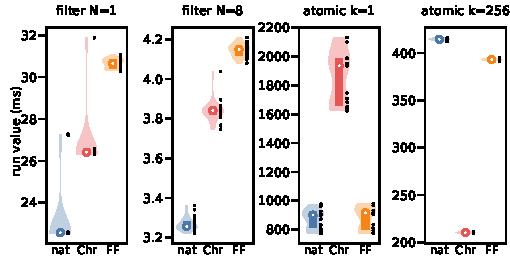
\includegraphics[width=0.9\linewidth]{../figures/campaign-distributions.pdf}
\caption{Distribution of the 30 per-run values of the filter and of the
atomic histogram, per environment.}
\Description{Violin plots of per-run medians for the filter and the atomic histogram in the three environments.}
\label{fig:distributions}
\end{figure}
